\documentclass[11pt, letterpaper]{article}

%%% compuerta logica, funcion booleana - tipos, pulldown
%%%
%paquetes
\usepackage{tikz}
\usepackage{xcolor}
\usepackage{graphicx}
\usepackage{amsmath}
\usepackage{amssymb}
\usepackage[utf8]{inputenc} % Tildes
\usepackage[spanish]{babel} % Language
\usepackage{babelbib} % Bibliografia español
\usepackage{colortbl}
\usepackage{float}
\usepackage{fancyhdr}
\usepackage{utilidades}
\usepackage[utf8]{inputenc}
\usepackage{lastpage}
\usepackage[right = 2.5 cm, left = 2.5 cm, top = 1.5 cm , bottom = 2 cm]{geometry}
\usepackage{enumitem} %sirve para cambiar el tipo de enumeracion si redefinir comandos ejem: \arabic* \alph*
\usepackage{karnaugh-map}
\usepackage{url}
\usepackage{hyperref}

%configuraciones
\graphicspath{{img/}}
\spanishdecimal{.}	
\pagestyle{fancy}
\fancyhf{}
\renewcommand{\headrulewidth}{0pt}
\hypersetup{colorlinks=true, linkcolor=black, urlcolor=black}

%%%%%%%%%%%%%%%%%%%%%%%%%%%%%%%%%%%%%%%%%%%%%%%%%%%%%%%%%%%%%%%%%%%%%%%%%%
%%%%%%%%%%%%%%%%%%%%%%% DOCUMENT BODY %%%%%%%%%%%%%%%%%%%%%%%%%%%%%%%%%%%%
%%%%%%%%%%%%%%%%%%%%%%%%%%%%%%%%%%%%%%%%%%%%%%%%%%%%%%%%%%%%%%%%%%%%%%%%%%	

\begin{document} 
	%%%%%%%%%%%%%%%%%%%%%%%%%%%%%%%%%%%%%
	%%%%%%%%%%%%% HEADER %%%%%%%%%%%%%%%%
	%%%%%%%%%%%%%%%%%%%%%%%%%%%%%%%%%%%%%
	%%%% BLOQUE DE DATOS %%%
\newcommand{\Title}{
	Práctica de Laboratorio \#3
	Multiplexores
} %Titulo del reporte

\newcommand{\LogoUniversity}{img/logo.jpg} %localizacion del logo
\newcommand{\NameUniversity}{Universidad Galileo} %Nombre de la universidad
\newcommand{\Date}{
	Guatemala, 6 de marzo de 2020
} %Fecha de entrega
\newcommand{\Faculty}{Facultad FISICC} %Nombre de la facultad
\newcommand{\Course}{
	Curso: Sistemas de Arquitectura
} %Nombre del curso
\newcommand{\ID}{
	Carnet: 1800 2955
}
\newcommand{\Student}{
	Alumno: Josu\'e Benyamin Isa\'i Galeano Morales
} %Nombre del estudiante
\newcommand{\Section}{
	Secci\'on: A
} %Sección del estudiante
\newcommand{\Schedule}{
	Horario de laboratorio: 18:00 a 19:00
} %Horario
\newcommand{\Assistant}{
	Auxiliar: Evelyn Cruz
} %Persona encargada
\newcommand{\Day}{
	Día de laboratorio: viernes
} %Dia en que recibe
%% FIN BLOQUE DE DATOS%%


%% NO ES NECESARIO MODIFICAR ESTA PARTE %%
\textbf{
	\small
	\hspace{-1 cm}
	\begin{minipage}{0.15\textwidth}
		%%%%%%%%%%%%%%%%% LOGO %%%%%%%%%%%%%%%%%%%%%%%%%%%%%%%
		\includegraphics[scale=0.5]{\LogoUniversity}
	\end{minipage}
	\begin{minipage}{0.7\textwidth}
		\resizebox{1.25\textwidth}{!}{
			\begin{tabular}{ll}
				\hline 
				%%%%% PARTE SUPERIOR DE LA TABLA DE DATOS %%%%%%%%%%%%%%%%%%%%%%%
				\NameUniversity & \Date \\
				\hline
				\rowcolor{lightgray}
				\Faculty & \Student\\
				\hline 
				\Course & \ID\\
				\hline\rowcolor{lightgray}
				\Section & \Schedule\\
				\hline 
				\Assistant & \Day\\
				\hline
			\end{tabular}
		}
	\end{minipage}
}

\vspace{0.5cm}
\begin{tikzpicture}
\hspace{-1 cm}
\draw (0.1,0.1) rectangle (1.043\textwidth,0.9);
\draw[line width=0.7mm] (0,0) rectangle (1.05\textwidth,1);
\node[font=\Large] at (0.525\textwidth, 0.45) {\textbf{\Title}};
\end{tikzpicture}		

\vspace*{0.5 cm}
 %incluimos la parte del header en el documento, note que header es como escribir dentro de un ambiente document por lo tanto no debe llevar definición de clase ni definiciones que se hagan exclusivamente en el preambulo.
		
	\begin{block}{Objetivos:}
		\begin{enumerate}
			\item Que el estudiante se familiarice con el funcionamiento de un multiplexor y que logre
			diseñar y construir lógica combinacional con dispositivos de mediana integración.
		\end{enumerate}
	\end{block}

	\begin{block}{Materiales:}
		\begin{enumerate}
			\item Fuente de 5VDC (Proporcionada por el Laboratorio).
			\item Punta Lógica.
			\item 1 Bread Board.
			\item Pinzas para cortar y pelar alambre.
			\item 1 metro de cable UTP.
			\item 1 DIP switch de 4 polos.
			\item 1 Circuito Integrado 74LS151.
			\item 1 LED Rojo.
			\item 1 Resistor de 180k$\Omega$.
			\item 3 Resistores de 10k$\Omega$
		\end{enumerate}
	\end{block}

	\begin{block}{Resumen:\\}
		
		En base al diagrama entregado para hacer el laboratorio, se buscó información del IC 74LS151 tipo N y en base al diagrama se construyó dicho circuito, por la forma construcción que se empleo el led encendía con 0s lógicos y es por esto que se tomó la salida negada para obtener dicho comportamiento.
	\end{block}

	\begin{block}{Marco Teórico:\\}
		
		Los \textbf{Multiplexores} son circuitos combinacionales que tienen la característica dejar pasar una señal de las $2^n$ señales en función de sus $n$ selectores, se utilizan para ``colar'' la información. Como es de suponer sólo tiene una salida que resulta ser la seleccionada por los selectores. Este es un caso particular de los decodificadores.
		\newpage
		
		\begin{figure}[H]
			\Center{
				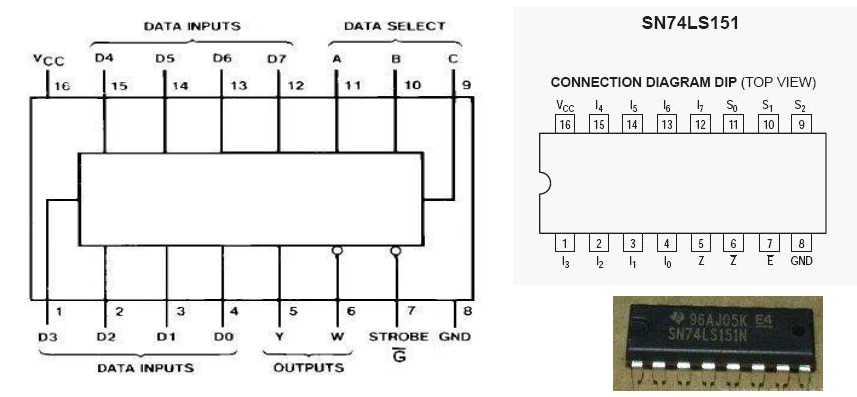
\includegraphics[scale=.6]{multiplexor}
				\caption{Información de \textbf{SN74LS151} multiplexor empleado para el laboratorio}
			}
		\end{figure}
		
	\end{block}

	\begin{block}{Datos Prácticos:\\}
		 \begin{figure}[H]
		 	\def\arraystretch{1.5}
		 	\Center{
		 		\begin{tabular}{|c|c|c|c|}
		 			\hline
		 			\multicolumn{3}{|c|}{\textbf{Entradas}}&\multicolumn{1}{|c|}{\textbf{Salidas}}\\
		 			\hline
		 			\textbf{$D_0$}&\textbf{$D_1$}&\textbf{$D_2$}&\textbf{LED}\\
		 			\hline
		 			0 &	0 &	0 &	1\\
		 			0 &	0 &	1 &	0\\
		 			0 &	1 &	0 &	1\\
		 			0 &	1 &	1 &	1\\
		 			1 &	0 &	0 &	0\\
		 			1 &	0 &	1 &	0\\
		 			1 &	1 &	0 &	0\\
		 			1 &	1 &	1 &	1\\
		 			\hline
		 		\end{tabular}
		 	}
		 	\caption{tabla de comportamiento del LED}
		 \end{figure}
  	
  		\begin{figure}[H]
			\Page{.5}{
				\Center{
					\begin{karnaugh-map}[4][2][1][$D_1D_0$][$D_2$]
						\minterms{0,2,3,7}
						\implicant{3}{7}
						\implicantedge{0}{0}{2}{2}
					\end{karnaugh-map}
				}
				\caption{mapa de karnaugh}
			} \Page{.5}{
				\Center{
					$$\displaystyle\bar{D_2}\bar{D_0}+D_1D_0$$
				}
				\caption{Expresión}
			}
  		\end{figure}
	\end{block}

	\begin{block}{Conclusiones:\\}
		\begin{enumerate}
			\item Poder elegir entre múltiples señales es muy importante cuando se diseñan arquitecturas.
			\item Los multiplexores pueden ser utilizados para obtener una lectura entre varios flip-flops y así poder obtener una palabra en especifico.
		\end{enumerate}
	\end{block}

	\bibliographystyle{apalike}
	\bibliography{referencias}
	\nocite{*}
	
\end{document}
